%% chapter06_agency_slides.tex
%% Beamer slides for Chapter 6: Agency
%% "An Introduction to Universal Artificial Intelligence"
%% by Marcus Hutter, Elliot Catt, and Jordi Grau-Moya (CRC Press / Chapman & Hall, 2024)
%% Sections covered: 6.1 - 6.9 (complete chapter)
%% Reader-friendly style: complete sentences, symbol explanations, worked examples.
%% Compiled with: pdflatex -interaction=nonstopmode chapter06_agency_slides.tex  (twice)
\documentclass[aspectratio=169,10pt]{beamer}

\usetheme{Madrid}
\usecolortheme{seahorse}
\usefonttheme{professionalfonts}

%% ── Packages ──────────────────────────────────────────────────────────────
\usepackage{amsmath,amssymb,amsfonts}
\usepackage{mathtools}
\usepackage{graphicx}
\usepackage{booktabs}
\usepackage{array}
\usepackage{xcolor}
\usepackage{listings}
\usepackage{stmaryrd}

\graphicspath{{figures/}}

%% ── Python listing style ─────────────────────────────────────────────────
\lstdefinestyle{pycode}{
  language=Python,
  basicstyle=\ttfamily\scriptsize,
  numbers=left,
  numberstyle=\tiny\color{gray},
  frame=single,
  backgroundcolor=\color{gray!7},
  keywordstyle=\color{blue!70!black}\bfseries,
  commentstyle=\color{green!50!black}\itshape,
  stringstyle=\color{orange!80!black},
  showstringspaces=false,
  breaklines=true,
  tabsize=2,
  xleftmargin=1.0em,
  framexleftmargin=1.0em,
  aboveskip=4pt,
  belowskip=4pt,
}
\lstset{style=pycode}

%% ── Convenience macros ───────────────────────────────────────────────────
\newcommand{\A}{\mathcal{A}}
\newcommand{\Ocal}{\mathcal{O}}
\newcommand{\Rcal}{\mathcal{R}}
\newcommand{\Ecal}{\mathcal{E}}
\newcommand{\Hcal}{\mathcal{H}}
\newcommand{\histlt}{h_{<t}}

%% ── Metadata ─────────────────────────────────────────────────────────────
\title[UAI -- Ch.6]{An Introduction to Universal Artificial Intelligence}
\subtitle{Chapter 6: Agency}
\author{Based on Hutter, Catt \& Grau-Moya}
\institute{CRC Press / Chapman \& Hall, 2024}
\date{}

\setbeamertemplate{footline}[frame number]
\setbeamertemplate{navigation symbols}{}

%% ══════════════════════════════════════════════════════════════════════════
\begin{document}

\begin{frame}
  \titlepage
\end{frame}

\begin{frame}{Outline}
  \tableofcontents
\end{frame}

%% ══════════════════════════════════════════════════════════════════════════
\section{Chapter Overview}
%% ══════════════════════════════════════════════════════════════════════════

\begin{frame}[allowframebreaks]{Chapter 6: Agency --- Why Do We Need It?}

Up until this point in the book, the discussion has been about how to
\emph{predict} well. A predictor that only watches and forecasts what
happens next, without changing what happens, is called a \emph{passive
agent}: it already has all the information it needs in order to predict,
and its guesses do not feed back into the world. For an artificial
intelligence to actually have an impact on its environment, it needs
\emph{agency}: the ability to choose actions that change what happens next.

\vspace{0.3cm}
An \emph{active agent}, or simply \emph{agent}, is something that
interacts with the environment, and for which the environment's future
behavior depends not only on past events, but also on what the agent
chooses to do.

\vspace{0.3cm}
\textbf{This chapter builds a complete framework for agency:}
\begin{itemize}
  \item \textbf{6.1 Policy and Environment.} How do we formalize an agent
    and the environment it interacts with?
  \item \textbf{6.2 Assigning Rewards.} How do we measure whether the agent
    is doing a good job?
  \item \textbf{6.3 (PO)MDP vs.\ History RL.} How does our general
    history-based setup relate to the standard Markov Decision Process
    framework used throughout reinforcement learning?
  \item \textbf{6.4 Time Discounting.} Why does naively summing all future
    rewards break down, and how do we fix it by valuing the present more
    than the future?
  \item \textbf{6.5 Time Consistency.} Which discounting schemes keep an
    agent's plans stable as time passes, and which cause pathological
    behavior?
  \item \textbf{6.6 Value Functions.} How ``good'' is a given situation for
    the agent, defined recursively via the Bellman equation?
  \item \textbf{6.7 Q-Value.} How good is it to take a specific action right
    now, and how does this connect back to the value function?
\end{itemize}

\framebreak

\textbf{Epigraph of this chapter} (Clifford Ambrose Truesdell):
\begin{quote}
\itshape ``There is nothing that can be said by mathematical symbols and
relations which cannot also be said by words. The converse, however, is
false. Much that can be and is said by words cannot be put into equations,
because it is nonsense.''
\end{quote}

\vspace{0.3cm}
\textbf{A note on scope.} This chapter pursues a \emph{history-based}
approach to reinforcement learning (RL), which is more general than the
standard Markov Decision Process (MDP) presentation. Readers unfamiliar with
the standard MDP treatment of reinforcement learning are still encouraged to
familiarize themselves with it, e.g.\ via Sutton \& Barto's textbook
(cited in the book as [SB18], Chapter 3), since many algorithms and
intuitions in the wider field are phrased in MDP language.

\vspace{0.3cm}
\textbf{Roadmap of ideas.} We first formalize what an agent is and how it
interacts with an environment (6.1). We then discuss how to measure the
agent's performance using scalar rewards (6.2), and how our general setup
relates to (PO)MDPs (6.3). Naively summing all future rewards can give an
undefined (infinite) measure of success, which motivates \emph{time
discounting}, i.e.\ valuing the present more than the future (6.4), and
raises the question of \emph{time consistency}: does an optimal plan stay
optimal as time passes (6.5)? We then define the \emph{value function},
capturing how good a situation is for the agent, expressed recursively via
the Bellman equation (6.6), and finally the \emph{Q-value}, capturing how
good a specific action is (6.7).
\end{frame}

%% ══════════════════════════════════════════════════════════════════════════
\section{6.1 Policy and Environment}
%% ══════════════════════════════════════════════════════════════════════════

\begin{frame}[allowframebreaks]{6.1 The Cybernetic Model}

We first discuss the \emph{cybernetic model}, the standard formal framework
used in reinforcement learning (RL) to reason about an agent interacting
with the world. The cybernetic model has two parts:

\begin{itemize}
  \item The \textbf{agent}, who observes what happens around it and makes
    decisions.
  \item The \textbf{environment}, the world with which the agent
    interacts.
\end{itemize}

The cybernetic model operates in discrete time, with the agent and
environment taking turns. At time $t$, the agent receives a \emph{percept}
$e_{t-1}$ from the environment, and responds in turn with an
\emph{action} $a_t$. The environment receives the action, and issues a new
percept $e_t$, and so on. Both the percepts issued by the environment and
the actions taken by the agent may depend on the entire \emph{history} (the
sequence of past action-percept interactions), and both the agent and
environment are permitted to be stochastic (random).

\vspace{0.2cm}
\begin{block}{Definition 6.1.1 (Stochastic function)}
A \emph{stochastic function}, or \emph{probability kernel}, or
\emph{conditional distribution} $f$ from $A$ to a countable set $B$,
denoted $f: A \to \Delta B$, is a function from $A$ to the set of all
probability distributions on $B$, denoted
$\Delta B := \{p \in [0,1]^B : \sum_{b \in B} p_b \le 1\}$. We define
$p(b|a) := f(a)_b$, the probability that the stochastic function $p$
returns $b$ given $a$ as input. If $x$ is sampled from a conditional
distribution $p(\cdot|a)$, we write $x \sim p(\cdot|a)$.
\end{block}

\textbf{Plain-English explanation.} A stochastic function does not return
one fixed answer for a given input; instead, it returns a whole probability
distribution over possible answers. $\Delta B$ is just notation for ``the
set of all probability distributions over $B$''. $p(b|a)$ reads as ``the
probability of getting output $b$ given input $a$''. The symbol $\sim$
(read ``is distributed as'' or ``is sampled from'') means that $x$ is drawn
at random according to that distribution.

\framebreak

\textbf{Action, percept, observation, reward, history spaces.} Formally, we
define:
\begin{itemize}
  \item $\A$ (script A) --- the set of \emph{actions} from which the agent
    can choose.
  \item $\Ocal$ (script O) --- the set of possible \emph{observations}.
  \item $\Rcal$ (script R) --- the set of possible \emph{rewards}.
\end{itemize}
The percept $e$ that the environment generates is an (observation, reward)
pair $(o,r)$. The set of all percepts is denoted
$\Ecal := \Ocal \times \Rcal$ (script E). Unless otherwise stated, the
following global assumptions are made.

\begin{block}{Assumption 6.1.2 (Finite action, observation, and reward spaces)}
We assume that the action, observation, and reward spaces $\A, \Ocal,
\Rcal$ (and therefore $\Ecal$) are finite. For simplicity we also assume
that the rewards are bounded between $0$ and $1$.
\end{block}

\textbf{Why bound rewards in $[0,1]$?} The requirement $r_k \in [0,1]$ is
often relaxed when presenting examples. For finite $\Rcal$, the rewards are
bounded, and can always be rescaled to fit in $[0,1]$ via an affine
(``stretch and shift'') transformation. This rescaling does not change
which policy is optimal for that environment (though there is a subtlety
covered in an exercise later in the book).

\begin{block}{Remark 6.1.3 (Infinite spaces)}
Many statements could be generalized to infinite spaces, but from an AI
perspective this does not lead to interesting additional insights, and only
unnecessarily complicates the mathematics. For countable spaces, $\max$
becomes $\sup$ (supremum, the least upper bound) and $\operatorname{argmax}$
must be replaced by $\varepsilon$ (epsilon)-optimal choices, and sums need
convergence checks. Uncountable spaces need topology and measure-theoretic
assumptions; sums $\sum$ become integrals $\int$.
\end{block}

\framebreak

\textbf{Histories.} A history is a finite sequence of action-percept pairs.
The set of all histories is $\Hcal := (\A \times \Ecal)^{*}$ (the star
means ``all finite sequences of''). The agent chooses an action using a
\emph{policy}, a stochastic function from histories to actions,
$\pi: \Hcal \to \Delta \A$. An \emph{environment} is a stochastic function
from a history plus the agent's last action to a percept,
$\nu: \Hcal \times \A \to \Delta \Ecal$ (or $\Delta' \Ecal$ for
\emph{chronological semimeasures}, defined later).

\vspace{0.2cm}
We write $h_{<t} := h_{1:t-1}$ for the history up to time $t-1$, that is,
\[
  h_{<t} \;:=\; a_1 e_1 a_2 e_2 \ldots a_{t-1} e_{t-1}
  \;=\; a_1 o_1 r_1 a_2 o_2 r_2 \ldots a_{t-1} o_{t-1} r_{t-1}.
\]
\textbf{Symbol-by-symbol.} $h_{<t}$ is ``the history strictly before time
$t$''. Each $a_i$ is the action chosen at step $i$, and each
$e_i = (o_i, r_i)$ is the percept (observation $o_i$ plus reward $r_i$)
returned by the environment right after that action.

We also sometimes use the shorthand
\[
  a_{1:t} = a_1 a_2 \ldots a_t \qquad \text{and} \qquad
  e_{1:t} = e_1 e_2 \ldots e_t = o_1 r_1 \ldots o_t r_t.
\]
These just concatenate all actions, or all percepts, from step $1$ up to
step $t$ inclusive.

\framebreak

\begin{block}{Definition 6.1.4 (Cybernetic model)}
We say an \emph{agent} interacts with an \emph{environment} in cycles
$t=1,2,\ldots$. In each cycle, the agent takes an action
$a_t \sim \pi(\cdot|h_{<t})$ sampled from its \emph{policy} given the
\emph{history} $h_{<t}$ as input. This action $a_t$ is given to the
environment, which generates a percept $e_t \sim \mu(\cdot|h_{<t}a_t)$
sampled from the environment distribution $\mu$ given the history $h_{<t}$
and the action $a_t$. The percept $e_t$ is passed to the agent, and the
next cycle $t+1$ begins. The percept
$e_t \equiv (o_t, r_t) \equiv o_t r_t \equiv or_t$ consists of a regular
\emph{observation} $o_t$ and a real-valued \emph{reward} $r_t$.
\end{block}

\begin{center}
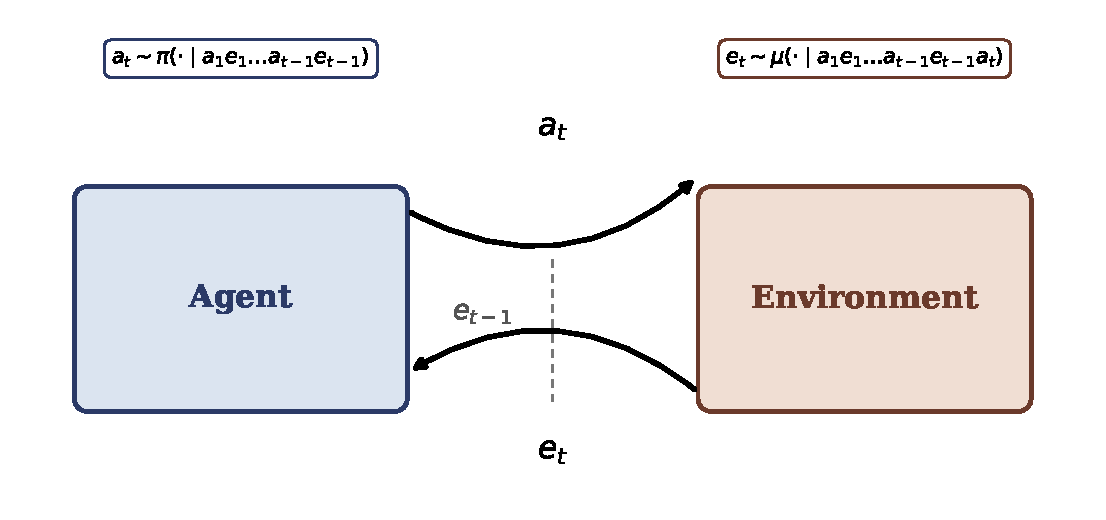
\includegraphics[width=0.72\textwidth]{cybernetic_model}
\end{center}

\textbf{Figure 6.1 (recreated).} An illustration of the cybernetic model.
The percept $e_{t-1}$ was generated in the previous cycle. In the current
cycle $t$, the agent takes action $a_t$ (top arrow), and the environment
reacts in turn with percept $e_t$ (bottom arrow). Both agent and environment
have access to the past sequence of actions and percepts, illustrated by
the thought-bubbles showing exactly what each side conditions on.

\framebreak

\textbf{Agent-environment interaction.} We usually denote the \emph{true}
underlying environment function by $\mu$ (mu), and use $\nu$ (nu) to denote
an \emph{arbitrary} environment distribution --- a hypothesis the agent
might entertain about how the world behaves. Usually $\mu$ is unknown to
the agent's policy $\pi$, and must be learned via interaction. Jointly,
$\nu$ and $\pi$ create the history.

\begin{block}{Definition 6.1.5 (Agent-environment measure $\nu^\pi$)}
The interaction between an environment $\nu$ and the policy $\pi$ induces a
probability measure $\nu^\pi : \Hcal \to [0,1]$ on histories (technically it
is a measure on cylinder sets). Conditioning on past history $h_{<t}$, we
have:
\[
  \nu^\pi(h_{t:m}|h_{<t}) \;:=\; \prod_{k=t}^{m} \pi(a_k|h_{<k})\,\nu(e_k|h_{<k}a_k)
\]
\end{block}

\textbf{Plain-English explanation.} $\nu^\pi(h_{t:m}|h_{<t})$ is the
probability of observing the particular stretch of history $h_{t:m}$ (from
step $t$ to step $m$) given everything that happened before time $t$. It
factors into a product over each time step $k$: the probability $\pi$
assigns to the action actually taken at step $k$, multiplied by the
probability $\nu$ assigns to the percept actually received at step $k$.
This is nothing but the chain rule of probability, applied one action and
one percept at a time.

\framebreak

\begin{block}{Remark 6.1.6 (Lifting sequence prediction to interacting agents)}
Many definitions and results in this chapter mirror those from the
sequence-prediction setting covered earlier in the book. Definition 6.1.5
is just the chain rule $\rho(x_{1:n}) = \prod_{t=1}^{n} \rho(x_t|x_{<t})$
for $\mathcal{X} = \A \times \Ecal$, further factorizing $a_k e_k$ and
$\rho$ into $\pi$ and $\nu$. For one-step prediction with a fixed policy
$\pi$, all concepts and results for a predictor $\xi$ (xi) essentially carry
over to $\xi^\pi$. When comparing different policies of far-sighted agents,
matters become much more intricate.
\end{block}

\begin{block}{Definition 6.1.7 (Probability measure $\mathrm{P}^\pi_\nu$ and expectation $\mathrm{E}^\pi_\nu$)}
Let $\mathrm{P}^\pi_\nu[Q|h_{<t}]$ denote the probability of some measurable
predicate or event $Q \subseteq (\A \times \Ecal)^\infty$, where the future
histories $h_{t:m}$ given past history $h_{<t}$ are sampled from
$\nu^\pi(h_{t:m}|h_{<t})$. Similarly, the (conditional) expectation
$\mathrm{E}^\pi_\nu[f|h_{<t}]$ of some measurable function
$f: (\A\times\Ecal)^\infty \to \mathbb{R}\cup\{\pm\infty\}$ is the
expectation with respect to the (conditional) probability measure induced
by $\nu^\pi$. For events $Q_m = Q'_m \times (\A\times\Ecal)^\infty$ with
$Q'_m \subseteq (\A\times\Ecal)^m$ and functions
$f_m : (\A\times\Ecal)^m \to \mathbb{R}$, explicit expressions are
\[
  \mathrm{P}^\pi_\nu[Q_m|h_{<t}] = \sum_{h_{t:m}:h_{t:m}\in Q_m} \nu^\pi(h_{t:m}|h_{<t})
  \qquad
  \mathrm{E}^\pi_\nu[f_m|h_{<t}] = \sum_{h_{t:m}} \nu^\pi(h_{t:m}|h_{<t}) f(h_{1:m})
\]
\end{block}

\textbf{Plain-English explanation.} $\mathrm{P}^\pi_\nu$ (the probability
measure induced by policy $\pi$ and environment $\nu$) and $\mathrm{E}^\pi_\nu$
(the corresponding expectation, i.e.\ average value) let us talk formally
about ``the probability of some event occurring'' or ``the expected value
of some quantity'' once we fix how the agent behaves ($\pi$) and how the
world responds ($\nu$). We have
$\mathrm{P}^\pi_\nu[h_{1:m}|h_{<t}] = \nu^\pi(h_{t:m}|h_{<t})$ by definition,
which proves the explicit expressions above. Existence and uniqueness of
this measure for any event $Q$ follows from a standard result in measure
theory (the Carath\'eodory Extension Theorem).

\framebreak

\textbf{History-based reinforcement learning.} The policy and the
environment interact with each other and create a history, as choices made
by the policy affect what future percepts (observations, rewards) the
environment will generate. This setup is called \emph{history-based
reinforcement learning} or \emph{general reinforcement learning}. We
consider the scenario where the dynamics of the environment are unknown to
the agent, and the agent must learn the underlying stochastic function
$\mu$ that governs the environment, while also trying to perform well ---
that is, take actions that cause the environment to return large rewards.

\begin{block}{Exploration-exploitation tradeoff}
For the agent to learn $\mu$, it must sometimes take suboptimal actions
which may not immediately maximize the expected reward based on the
agent's current belief about the environment, but which will allow the
agent to gain more confidence about which environment it is actually in.
For the agent to perform well in the environment means to maximize the
(expected future) reward. These are often conflicting goals.
\end{block}

\textbf{Plain-English explanation.} \emph{Exploration} means improving the
current belief about what environment the agent is in (e.g.\ trying new
actions to learn more). \emph{Exploitation} means maximizing reward based on
what environment the agent currently believes it is in (e.g.\ repeating
known-good actions). An agent that explores too much acts suboptimally
because it keeps testing things instead of collecting reward, while an
agent that exploits too much never fully understands the environment's
dynamics and so never discovers how to act truly optimally.
\end{frame}

\begin{frame}[fragile]{Python: Simulating the Cybernetic Model}
The following toy example simulates the agent-environment loop of
Definition 6.1.4 for a simple stochastic environment (a biased two-armed
bandit hidden inside the history-based framework), tracking the actual
numeric history and rewards produced.

\begin{lstlisting}
import random
random.seed(0)

# Two actions: 'L' (left arm) and 'R' (right arm).
# True environment mu: reward 1 with prob 0.3 for L, prob 0.7 for R.
A = ['L', 'R']
true_reward_prob = {'L': 0.3, 'R': 0.7}

def mu(action):
    # e_t = (o_t, r_t); here o_t is trivial (always 'ok')
    r = 1 if random.random() < true_reward_prob[action] else 0
    return ('ok', r)

def pi(history):
    # Simple epsilon-greedy policy learned online from history
    counts = {a: 0 for a in A}
    totals = {a: 0 for a in A}
    for (a, e) in history:
        counts[a] += 1
        totals[a] += e[1]
    if random.random() < 0.1 or min(counts.values()) == 0:
        return random.choice(A)          # explore
    avg = {a: totals[a] / counts[a] for a in A}
    return max(avg, key=avg.get)          # exploit

history = []            # h_{<t} as a Python list of (a_k, e_k) pairs
total_reward = 0
for t in range(1, 21):
    a_t = pi(history)               # a_t ~ pi(.|h_{<t})
    e_t = mu(a_t)                   # e_t ~ mu(.|h_{<t} a_t)
    history.append((a_t, e_t))
    total_reward += e_t[1]
    print(f"t={t:2d}  a_t={a_t}  e_t={e_t}  cumulative reward={total_reward}")
\end{lstlisting}

\textbf{What this shows.} At every cycle $t$, the policy \texttt{pi} looks
only at the history so far (an epsilon-greedy strategy that mostly exploits
the arm with the best observed average reward, but explores 10\% of the
time), producing $a_t$; the environment \texttt{mu} then samples $e_t$
given $a_t$. After 20 cycles the policy typically converges to preferring
action \texttt{'R'}, since its true reward probability (0.7) exceeds
\texttt{'L'}'s (0.3) --- but only because it explored enough early on to
discover this, illustrating the exploration-exploitation tradeoff.
\end{frame}

%% ══════════════════════════════════════════════════════════════════════════
\section{6.2 Assigning Rewards}
%% ══════════════════════════════════════════════════════════════════════════

\begin{frame}[allowframebreaks]{6.2 Assigning Rewards}

We also need to define what it means for an agent to \emph{perform well}.
Later in the book, different ways of measuring performance using
\emph{utility functions} are discussed, but for now the focus is solely on
agents whose goal is to maximize the expected value of the sum of all
future rewards.

\begin{block}{Assumption 6.2.1 (Reward Hypothesis)}
``All of what we mean by goals and purposes can be well thought of as
maximization of the expected value of the cumulative sum of a received
scalar signal (called reward).'' (Sutton \& Barto, [SB18])
\end{block}

\textbf{Chess example.} Given an agent playing chess, the set of actions
available are legal chess moves, the observation is the current state of
the board, and the environment returns a new board where the opposing
pieces have made a legal move (the environment effectively hides the
opponent player). The environment's moves could come from an existing chess
engine, or from self-play. The reward could be: $+1$ if the agent's
previous action checkmated the enemy king; $-1$ if the new board places the
agent's own king in checkmate; and $0$ otherwise. This reward scheme aligns
with the correct behavior: to maximize the expected future reward sum, the
agent should take actions that lead to higher confidence of winning, and
avoid actions that lead to a loss.

\vspace{0.2cm}
But these rewards are \emph{sparse}: the agent receives a reward very
rarely, only when the game terminates, so it may take a very large number
of interaction cycles for the agent to learn to play chess well.

\framebreak

\textbf{The difficulty of sparse rewards.} Imagine trying to learn chess by
being sat down in front of a board, not knowing the rules or strategy of
the game (or even what the goal is!), and then randomly playing moves. The
only feedback is a scolding if you lose (or play an illegal move), and
praise if you win. It would not be surprising if even learning the rules
this way was difficult, let alone becoming proficient at the game (though
there is a documented strong counter-argument in the literature, [Hut05b,
Sec.6.3.4]).

\begin{block}{Reward shaping}
One potential solution to sparse rewards is to \emph{shape} the reward
function, offering small rewards for observations that are expected to be
strongly correlated with achieving the goal. For chess: capturing pieces,
avoiding having your own pieces captured, having pieces with a large
degree of freedom of where to move, controlling the center of the board,
and pinning enemy pieces are all strategies that positively correlate with
winning.
\end{block}

\textbf{Instrumental vs.\ terminal goals.} Bostrom calls these sub-goals
\emph{instrumental goals}: goals that often correlate with success and can
be used as a (often crude) proxy in service of the \emph{terminal goal} or
\emph{final goal}. In chess, the terminal goal is to win the game; all else
is secondary --- it does not matter to the agent how much material or
territory control is lost if a checkmate can be secured.

\framebreak

\begin{block}{Reward misspecification}
Shaping the reward can speed up learning, but it can also potentially lead
to a situation where the agent learns to ``game'' the shaped reward, by
exploiting the rewards for actions that correlate with the goal, rather
than trying to achieve the goal itself. For example, if there was too large
a reward associated with territorial control, the agent might try to move
pieces to lock down a large portion of the board and play too defensively,
rather than making moves with the objective of winning the game. This is
called \emph{reward misspecification}.
\end{block}

\textbf{The problem of teaching the rules.} There is also the problem of
how to teach the agent the rules of the game. The framework presented here
requires the agent to always select an action from a fixed action space
$\A$, but in chess the set of legal actions can vary from move to move.
This presents a dilemma: we would want the agent to be able to learn how to
play chess from interaction with the environment alone, rather than
hardcoding the rules of the environment into the agent, since the latter
would make the agent specific to a particular environment, and subvert the
purpose of \emph{universal} artificial intelligence. On the other hand,
with a fixed action space $\A$ containing all legal chess moves as a
subset, many of those moves would be illegal, depending on the current
state of the board.

\framebreak

\textbf{Handling illegal moves.} One solution is to allow illegal moves to
be part of the game, and whenever an illegal move is made, issue a reward
at least as bad as a loss to the agent. For games of a fixed length, the
penalty from an illegal move can take a while to learn from, since it may
be hard for the agent to distinguish illegal moves from legal but
suboptimal moves. A better approach is to \emph{terminate the game
immediately} upon playing an illegal move, and issue a penalty. When the
agent first begins interaction with the environment, it will likely take
many illegal actions (and receive the associated penalty) until it stumbles
across a legal move. In this way, the agent can quickly learn what moves
are legal, and implicitly learn the rules of chess.

\vspace{0.2cm}
It is important that the reward of making an illegal move is at least as
bad as a loss; otherwise the agent could escape a doomed position by making
an illegal move. (For a similar reason, the penalty for humans caught
cheating in a game is usually higher than that of a loss, as otherwise
cheating would be a rational action from an otherwise lost position.)
\end{frame}

%% ══════════════════════════════════════════════════════════════════════════
\section{6.3 (PO)MDP vs.\ History RL}
%% ══════════════════════════════════════════════════════════════════════════

\begin{frame}[allowframebreaks]{6.3 The Markov Decision Process (MDP)}

Our history-based setup is quite different from the traditional MDP
(Markov Decision Process) setup, where the environment is assumed to be
\emph{Markov}: that is, the environment $\mu$ has the property that it only
depends on the \emph{last} observation produced and action taken, not the
entire history.

\begin{block}{Markov assumption}
\[
  \mu(e_t | h_{<t} a_t) \;=\; \mu(e_t | o_{t-1} a_t)
\]
\end{block}

\textbf{Plain-English explanation.} No matter how long the history $h_{<t}$
actually is, the probability of the next percept $e_t$ depends only on the
most recent observation $o_{t-1}$ and the action $a_t$ just taken --- all
earlier history is irrelevant. In the MDP framework, observations are
usually called \emph{states} and denoted $s_t$, but this chapter keeps
$o_t$ for consistency with the more general history-based framework. Hence
for MDPs, $\mu: \Ocal \times \A \to \Delta\Ecal$.

\vspace{0.2cm}
Since the past history is irrelevant to the behavior of the environment,
the optimal action also does not need to depend on it, so it suffices to
consider \emph{Markov policies}:
\[
  \pi(a_t|h_{<t}) \;=\; \pi(a_t|o_{t-1})
\]

\framebreak

\textbf{A subtlety about learning.} To clarify: the optimal agent
$\pi^{*}$ for any Markov environment is itself Markov, but the behavior of
an agent that \emph{learns} to optimize a policy out of the set of all
Markov policies (like Q-learning) is itself \emph{non-Markov}, as the
Q-value estimates are constructed from past experiences. In the MDP
framework, the policy may receive the same observation in multiple
different time steps, placing it essentially in the same situation as a
past interaction: a Markov policy is agnostic of how much time has passed,
or what the history was up to this point (though the optimization process
that chose this policy may be aware of the history so far). Most work and
major results in reinforcement learning take place in the MDP framework
[SB18]. The Markov assumption also means that the value function depends
only on the current observation (state), the choice of policy, and the MDP
dynamics. In the finite MDP case, the same state is visited repeatedly,
which makes it easier to devise learning algorithms.

\vspace{0.2cm}
\textbf{Classic MDP value function (preview of Section 6.6).} Given a
Markov environment $\mu$, the classic presentation of the value function
$V^\pi$ is defined as the expected sum of geometrically discounted future
rewards, given a discount factor $\gamma \in [0,1)$ (gamma; more on
discounting in Section 6.4):
\[
  V^{\pi}_{\mu,\gamma}(o_{t-1}) \;:=\;
  \mathrm{E}^\pi_\mu\!\left[\sum_{k=0}^{\infty} \gamma^k r_{t+k}\,\middle|\,o_{t-1}\right]
  \;=\;
  \sum_{a_t}\pi(a_t|o_{t-1})\sum_{o_t r_t}\mu(o_t r_t|o_{t-1},a_t)
  \Big(r_t + \gamma V^{\pi}_{\mu,\gamma}(o_t)\Big)
\]
where the second expression is the familiar recursive \emph{Bellman
equation}.

\textbf{Plain-English explanation.} $V^\pi_{\mu,\gamma}(o_{t-1})$ is ``how
much total (discounted) reward do I expect from now on, if I'm currently at
observation $o_{t-1}$ and follow policy $\pi$ in environment $\mu$''. The
Bellman equation says this value equals: the reward $r_t$ received right
now, plus $\gamma$ times the value of wherever I land next --- averaged
over the randomness in the agent's action choice and the environment's
response.

\framebreak

\begin{block}{Partially Observable Markov Decision Process (POMDP)}
A more general class of environments is \emph{Partially Observable Markov
Decision Processes} (POMDPs), where the environment is still Markov,
conditioned on the current \emph{state}, but the agent only receives an
\emph{observation} based on the state, not the state itself. Many states
may lead to the same observation, so the agent needs to infer what state
the environment is likely to be in, based on its observations so far, and
act accordingly.
\end{block}

\textbf{Example (maze navigation).} An agent trying to navigate a maze is a
natural POMDP: the observation is the nearby walls, while the (hidden)
state is the true location of the agent. The walls adjacent to the agent
give it some information about its location, but not enough to uniquely
determine it: a classic ``Cheese Maze'' benchmark environment with 11
distinct states (locations) maps down to only 5 distinct observations,
illustrating how much information is lost by observing walls instead of
the true location.

\vspace{0.2cm}
\textbf{History-based RL.} In history-based RL, any observation arbitrarily
far in the past may be potentially relevant for deciding the best action to
take now. As a result, no situation ever repeats exactly in history-based
RL, which renders most existing (Markov-specific) RL algorithms unsuitable.
This history-based setup is chosen because general agents need to be able
to handle such general environments. Indeed, this is the most general RL
setup, with both the MDP and the POMDP frameworks being special cases of
it: MDPs are the special case where the observation itself is Markov, and
POMDPs are the special case where a hidden Markov state exists but is only
partially revealed through the observation.

\framebreak

\textbf{Chronological environments and policies.} Environments $\nu$ are
called \emph{chronological}, in the sense that percepts received at time
$t$ depend only on histories taken at time $\le t$. In the way semimeasures
have been defined so far in the book, they are chronological by definition,
but in other presentations authors write $\nu(e_{1:t}||a_{1:t})$ (with a
double bar) to denote the probability that $\nu$ assigns to $e_{1:t}$
conditioned on $a_{1:t}$, while respecting the chronological requirement
that the probability assigned to percept $e_t$ cannot depend on actions
taken \emph{after} time step $t$ --- that is, future actions cannot affect
past percepts. Chronological policies are defined analogously.

\begin{block}{Definition 6.3.1 (Chronological semimeasures)}
Chronological environments/policies are semimeasures $\nu/\pi$ of history
$h_{1:t} \equiv a_1e_1 \ldots a_te_t$ that for all $t$ satisfy
\[
  \nu(e_{1:t}||a_{1:t}) = \prod_{i=1}^{t}\nu(e_i|h_{<i}a_i)
  \qquad\text{and}\qquad
  \pi(a_{1:t}||e_{<t}) = \prod_{i=1}^{t}\pi(a_i|h_{<i})
\]
\end{block}

\textbf{Plain-English explanation.} The double-bar notation
$\nu(e_{1:t}||a_{1:t})$ just packages up the same chain-rule factorization
seen earlier (Definition 6.1.5) into a single symbol emphasizing that the
whole percept sequence $e_{1:t}$ is conditioned on the whole action
sequence $a_{1:t}$, one step at a time, in chronological order.

\framebreak

Note that, on the other hand, \emph{any} joint semimeasure $\rho: \Hcal \to
[0,1]$ over actions \emph{and} percepts without any restrictions can be
decomposed as
\[
  \rho(h_{1:t}) = \nu(e_{1:t}||a_{1:t})\,\pi(a_{1:t}||e_{<t}) = \nu^\pi(h_{1:t})
  \tag{6.3.2}
\]

\textbf{Plain-English explanation.} Any way of jointly assigning
probabilities to a full sequence of actions and percepts can always be
split apart into ``the policy's part'' $\pi$ and ``the environment's part''
$\nu$, and reassembled exactly as the agent-environment measure $\nu^\pi$
from Definition 6.1.5.

\vspace{0.2cm}
\textbf{Deterministic policies and environments.} A policy is called
\emph{deterministic} if it only takes values $0$ or $1$ (i.e.\ it puts all
its probability mass on a single action). If a policy is deterministic, we
abuse notation and define $\pi(h_{<t}) := a_t$, where $a_t$ is the unique
action such that $\pi(a_t|h_{<t}) = 1$ (implicitly assuming the type
$\pi: \Hcal \to \A$). Deterministic environments are defined the same way:
we write $\nu(h_{<t}a_t) = e_t$ if $e_t$ is the unique percept that $\nu$
assigns probability $1$ to, given history $h_{<t}$ and action $a_t$.
\end{frame}

%% ══════════════════════════════════════════════════════════════════════════
\section{6.4 Time Discounting}
%% ══════════════════════════════════════════════════════════════════════════

\begin{frame}[allowframebreaks]{6.4 Motivation: Why Discount Rewards?}

All else being equal, humans prefer to receive rewards now rather than
later. If we believe that humans are rational agents, we may expect the
same to hold for artificial agents. If an agent maximizes the expected sum
of \emph{all} future rewards over an infinite number of time steps, the
agent may receive \emph{infinite} reward. However, an agent could perform
suboptimal actions (actions that are not optimal at that history/time step)
at every time step --- e.g.\ receiving only half the optimal reward per
time step --- which over infinite time steps is \emph{still} infinite
reward. Alternatively, the agent could procrastinate on its task for a few
thousand years, and then play optimally thereafter, and \emph{also} receive
infinite reward.

\vspace{0.2cm}
To the (undiscounted) agent, each of these strategies is equally valuable,
since they all lead to infinite reward, even though we would obviously not
prefer the agent to procrastinate or choose actions that receive
``less'' reward. Indefinite procrastination can even happen for
\emph{finite} total reward, illustrated later by the ``delay environment''
(Figure 6.3).

\vspace{0.2cm}
\textbf{Two fixes.}
\begin{itemize}
  \item Give the agent a finite lifespan, called a \emph{horizon}. The
    agent maximizes reward only over its finite lifespan. This can make
    the agent short-sighted if the horizon is short, or unsuitable for
    continuing tasks when the lifespan is not known in advance.
  \item \emph{Discount} the reward over time: make rewards later worth
    less than rewards now, by multiplying rewards with a discount
    function.
\end{itemize}

\framebreak

\begin{block}{Definition 6.4.1 (Discount function)}
A discount function is a function $\gamma: \mathbb{N}^+ \times
\mathbb{N}^+ \to \mathbb{R}$ with $\gamma(k,t) \ge 0$ and
$\forall t: \sum_{k=1}^{\infty}\gamma(k,t) < \infty$. Here $t$ represents
the current present time step during interaction, while $k \ge t$
represents the future time step the agent reasons about at time $t$. The
corresponding discount \emph{normalization factor} is defined as
$\Gamma_t := \sum_{k=t}^{\infty}\gamma(k,t)$.
\end{block}

\textbf{Plain-English explanation.} $\gamma(k,t)$ (gamma) is ``how much do
I weigh a reward received at future time $k$, when I am currently reasoning
from present time $t$''. It must be non-negative, and the total weight
summed over all future times must be finite --- otherwise the infinite
reward problem above resurfaces. $\Gamma_t$ (capital gamma) is just the
total weight of all future rewards from time $t$ onward, used later to
normalize the value function into a proper average. Often $\gamma$ does not
depend on $t$, in which case we write $\gamma_k := \gamma(k,t)$ and
$\Gamma_t = \sum_{k=t}^\infty \gamma_k$.

\vspace{0.2cm}
\textbf{Worked example.} An agent at current time step $t=3$ would discount
a reward $r_7$ received four steps further into the future ($k=7$) using
the weight $\gamma(7,3)$. Discount functions that depend on $t$ can be
\emph{time inconsistent} (Section 6.5).

\begin{center}
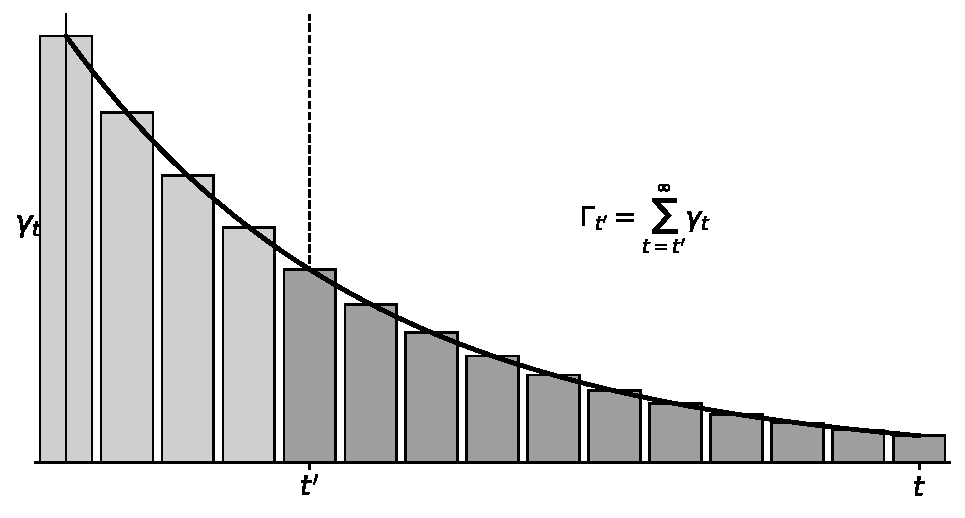
\includegraphics[width=0.62\textwidth]{discount_function}
\end{center}
\textbf{Figure 6.2 (recreated).} The discount function $\gamma_t$ (curve
and bars) and the normalizer $\Gamma_{t'} = \sum_{t=t'}^\infty \gamma_t$
(the shaded area under the bars from $t'$ onward).

\framebreak

\begin{block}{Definition 6.4.2 ($\varepsilon$-effective horizon)}
The $\varepsilon$-effective horizon $H_t(\varepsilon)$ at time $t$ is the
minimum number of time steps $k$ into the future such that the discount
factor $\Gamma_{t+k}$ is less than an $\varepsilon$ (epsilon) fraction of
the discount normalization factor $\Gamma_t$ at the present:
\[
  H_t(\varepsilon) \;:=\; \min_k \left\{ k \;\middle|\; \frac{\Gamma_{t+k}}{\Gamma_t} \le \varepsilon \right\}
\]
\end{block}

\textbf{Plain-English explanation.} $H_t(\varepsilon)$ answers: ``how far
into the future does the agent effectively look, before the remaining
future reward drops below a small fraction $\varepsilon$ of the total?''.
The \emph{effective horizon} is defined as $H_t(1/2)$: the earliest point
in time from which all potential reward from that point onward is worth
less than half of the potential reward available right now. It is a
tipping point summarizing how ``far-sighted'' the discount function makes
the agent.

\framebreak

\textbf{Discount function examples.} Readers familiar with the standard
MDP presentation of reinforcement learning will recognize the commonly
used \emph{geometric discount} function $\gamma_k = \gamma^k$ for some
$\gamma \in [0,1)$. One interpretation of this discount is that it behaves
as if the agent had a probability $1-\gamma$ of ``dying'' at each time step
(after which it receives a dummy percept forever and stops accumulating
reward). The geometric discount is also mathematically elegant, having the
property that $\Gamma_{k+1} = \gamma \Gamma_k$, which is convenient for MDP
RL.

\vspace{0.2cm}
Another choice is \emph{finite lifetime} discounting, where the agent does
not care about reward after a certain point $m$, that is,
$\gamma_k = \llbracket k \le m \rrbracket$ (the double brackets mean ``$1$
if the condition holds, else $0$''). This is equivalent to the agent having
a finite lifespan of $m$, and is effectively what happens in \emph{episodic
environments}, where interaction resets to some initial configuration after
at most $m$ time steps.

\vspace{0.2cm}
Similar to finite lifetime discounting is \emph{moving-horizon}
discounting, where the agent does not care about rewards beyond a finite
fixed horizon $m$, but the horizon itself moves with the current time step
$t$: $\gamma(k,t) = \llbracket t \le k \le t+m \rrbracket$.

\framebreak

\begin{table}[]
\centering
\scriptsize
\begin{tabular}{lccc}
\toprule
Discount & Param. & $\gamma_k$ & $\Gamma_k$ \\
\midrule
geometric & $\gamma\in[0,1)$ & $\gamma^k$ & $\dfrac{\gamma^k}{1-\gamma}$ \\[4pt]
finite life & $m\in\mathbb{N}_0$ & $\llbracket k\le m\rrbracket$ & $\max\{m-k+1,0\}$ \\[4pt]
power & $\delta>0$ & $\dfrac{1}{k^{1+\delta}}$ & $\dfrac{1}{\delta k^\delta}$ \\[4pt]
harmonic & $\delta>0$ & $\dfrac{1}{k(\ln k)^{1+\delta}}$ & $\approx \dfrac{1}{\delta(\ln k)^\delta}$ \\[4pt]
universal & -- & $2^{-K(k)}$ & decreases slower than any computable fn.\\[4pt]
no discount & -- & $1$ & $\infty$ \\
\bottomrule
\end{tabular}
\caption*{\scriptsize \textbf{Table 6.4} (abridged). $K(k)$ is the Kolmogorov
complexity of $k$ (length of the shortest program producing $k$), covered
earlier in the book. All rows are time-consistent except moving horizon
(omitted here; see Section 6.5).}
\end{table}

\textbf{Discount $\gamma(k,t) = (k-t+c)^{-1}$ (a cautionary example).} This
choice is undesirable, since it leads to time-inconsistent policies. Also,
the sum $\sum_{i=k}^\infty \gamma_i$ diverges, so it does not solve the
infinite reward problem; replacing exponent $-1$ by $-1-\delta$ for small
$\delta$ (delta) fixes the divergence (giving the ``power'' row above).

\vspace{0.2cm}
\textbf{The universal discount.} The universal discount
$\gamma_k = 2^{-K(k)}$ and its monotone variant $\gamma_k = \min_{i\le
k}2^{-K(i)}$ are the ``best'' in the sense that they lead to the most
far-sighted agent while ensuring $\Gamma_k$ does not diverge to infinity.
Being dependent on the Kolmogorov complexity $K$, however, makes this
discount factor \emph{incomputable}.
\end{frame}

\begin{frame}[fragile]{Python: Comparing Discount Functions}
This example computes and compares geometric, finite-life, and power
discount weights numerically, matching the structure of Table 6.4.

\begin{lstlisting}
import math

def geometric(k, gamma=0.85):
    return gamma ** k

def finite_life(k, m=8):
    return 1.0 if k <= m else 0.0

def power(k, delta=0.5):
    return 1.0 / k ** (1 + delta)

def normalizer(gamma_fn, k_start, n_terms=2000):
    return sum(gamma_fn(k) for k in range(k_start, k_start + n_terms))

for k in [0, 1, 2, 4, 8, 16]:
    print(f"k={k:2d}  geometric={geometric(k):.4f}  "
          f"finite_life={finite_life(k):.1f}  "
          f"power={power(max(k,1)):.4f}")

# Effective horizon H_0(0.5) for the geometric discount:
gamma = 0.85
Gamma0 = normalizer(lambda k: geometric(k, gamma), 0)
k = 0
while normalizer(lambda kk: geometric(kk, gamma), k) / Gamma0 > 0.5:
    k += 1
print(f"\nEffective horizon H_0(0.5) for gamma={gamma}: {k} steps")
\end{lstlisting}

\textbf{What this shows.} Running this prints, for a geometric discount
with $\gamma=0.85$, an effective horizon $H_0(0.5)$ of a handful of steps:
concretely, rewards more than roughly 4--5 steps into the future already
count for less than half of all remaining discounted value. This
quantifies, with real numbers, how ``far-sighted'' a given discount factor
actually is --- the qualitative idea behind Definition 6.4.2.

\begin{center}
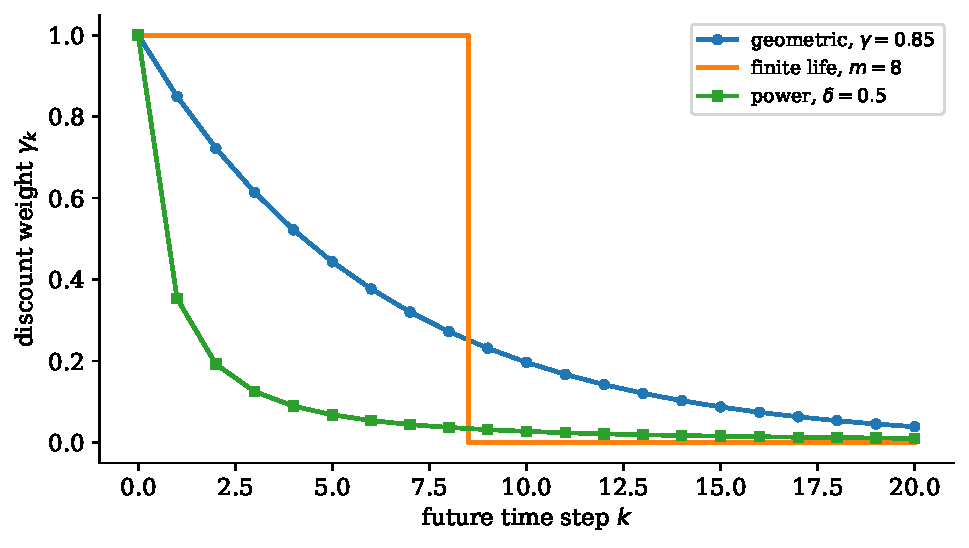
\includegraphics[width=0.6\textwidth]{discount_comparison}
\end{center}
\end{frame}

%% ══════════════════════════════════════════════════════════════════════════
\section{6.5 Time Consistency}
%% ══════════════════════════════════════════════════════════════════════════

\begin{frame}[allowframebreaks]{6.5 Time Consistency}

It seems sensible that once the best course of action by which an agent
will maximize expected discounted rewards has been determined, this plan
should not change once the future becomes the present (barring cases where
the agent has more information than when the plan was made). Discounts
that satisfy this property are called \emph{time-consistent} discounts.

\begin{block}{Theorem 6.5.1 (Time-consistent discounts)}
A discount function $\gamma(\cdot,\cdot)$ is \emph{time-consistent} if it
has no dependence on the present time step $t$. That is, $\gamma(k,t) =
\gamma_k$ for some function $\gamma: \mathbb{N}^+ \to \mathbb{R}$.
\end{block}

\textbf{Plain-English explanation.} If how much you discount a reward $k$
steps from now depends only on $k$ (how far away it is), and not on $t$
(what today's date happens to be), then your preferences about the future
never ``shift'' just because time has passed. That is exactly what
time-consistency means.

\framebreak

\begin{block}{Example 6.5.2 ((Un)healthy dinner)}
Humans are often time-inconsistent (children usually plan over shorter
timescales than adults), and the discount may even vary on timescales as
short as a few hours. For example, a person might convince themselves
early in the day to make something healthy for dinner that night. This
will incur negative rewards that evening due to the effort involved in
making dinner, but greater rewards in the long term due to health benefits.
Later that evening, they might shift to a more myopic (short-sighted)
discount, give up on making dinner and order take-out instead, which gives
large rewards immediately (take-out is delicious!) but less reward in the
long term, due to it being less healthy and costing more money than
homemade dinner.
\end{block}

\vspace{0.1cm}
Both geometric and finite lifetime discounting are time-consistent, but
\emph{constant horizon} discounting $\gamma(k,t) = \llbracket t \le k \le
t+m \rrbracket$ is \textbf{not}. This can lead to undesirable behavior
where the agent will forever delay current rewards in the hope of
receiving more reward later. In doing so, no reward is ever received.

\framebreak

\begin{center}
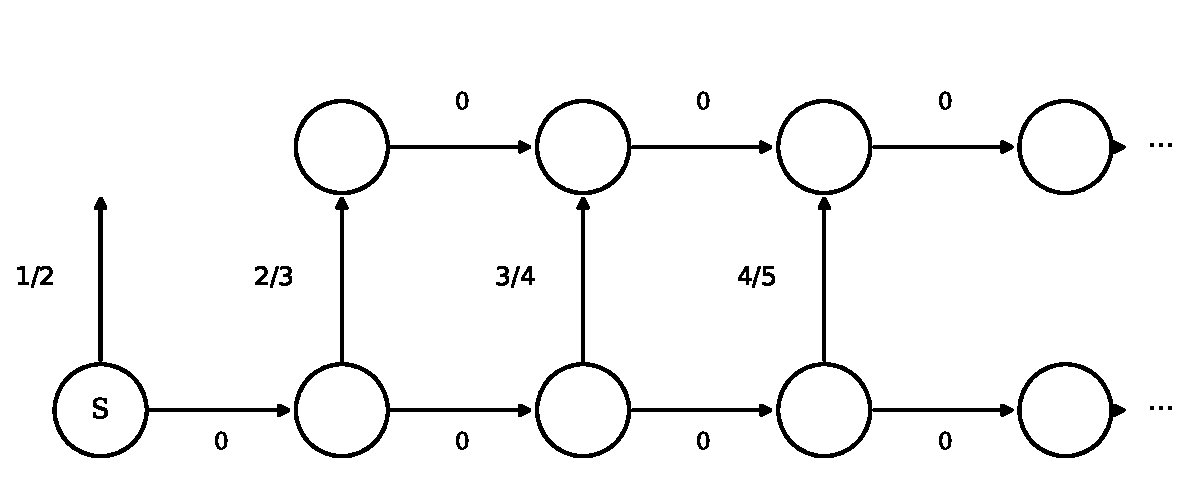
\includegraphics[width=0.85\textwidth]{delay_environment}
\end{center}
\textbf{Figure 6.3 (recreated).} The environment $\nu_{\text{delay}}$: from
each state the agent can choose to move \emph{up} to receive the associated
reward immediately, or move \emph{right} (reward $0$) to obtain more reward
later. A reward-maximizing agent with undiscounted infinite horizon or
finite moving horizon will delay reward forever and thus receive zero total
reward.

\begin{block}{Example 6.5.3 (Immortal and time-inconsistent agents)}
An agent interacting with $\nu_{\text{delay}}$ starts at the state marked
$S$. Given a moving horizon of $m=2$, the agent sees that it could move up
for reward $1/2$, or move right and then up for reward $2/3$ --- the only
rewards reachable within two time steps. Assuming the agent follows a
policy that maximizes the value function, it concludes the best action is
to move right. But once it does, the horizon has moved, and now it
considers moving up for $2/3$, or right and up for $3/4$. The agent
proceeds with this reasoning forever, always delaying potential reward now
for more reward later. As a result, the agent always moves right, and
receives reward zero forever. So the choice of a moving horizon means the
agent follows the \emph{worst} possible policy for this environment. This
remains true for any moving horizon $m \ge 2$ and infinite horizon.
\end{block}

\framebreak

\textbf{Contrast with time-consistent discounts.} Contrast the moving
horizon disaster with (any) finite lifetime $m$, where the agent will walk
$m-1$ steps to the right and then up, to receive an expected discounted
reward sum of $\frac{m}{m+1}$. Similarly, with geometric discounting for
some $\gamma \in [0,1)$, the agent will choose to walk $k^{*}-1$ steps
right, and then on time step $k^{*}$, walk up, where
\[
  k^{*} = \operatorname*{argmax}_{k\ge 1}\left\{\gamma^{k-1}\frac{k}{k+1}\right\} < \infty.
\]

\textbf{Plain-English explanation.} Unlike the moving horizon (which always
prefers to wait one more step, forever), both finite-lifetime and
geometric discounting eventually conclude that ``cashing in'' is better
than waiting even further, because the discount on far-future rewards
eventually outweighs the marginal gain $\frac{k}{k+1}$ from waiting one
more step. This gives a well-defined, finite optimal stopping point
$k^{*}$.

\vspace{0.2cm}
\textbf{Hyperbolic discounting in humans.} Based on psychology experiments
where humans are given the choice of some money now or more money later,
humans tend to discount hyperbolically (a discount shape between geometric
and power-law), a well-documented empirical finding.
\end{frame}

\begin{frame}[fragile]{Python: Moving Horizon vs.\ Geometric Discount in the Delay Environment}
This simulates the delay environment $\nu_{\text{delay}}$ and compares the
total reward actually collected under a moving-horizon policy (which always
delays) against a geometric-discount policy (which eventually cashes in).

\begin{lstlisting}
def reward_if_up_at_step(k):
    # reward for moving 'up' after k steps to the right: k/(k+1)
    return k / (k + 1)

# --- Moving horizon policy: always prefers "right" (delay) forever ---
# (Matches the book's proof: for any m >= 2, right is always weakly better.)
moving_horizon_reward = 0.0   # confirmed analytically: always 0

# --- Geometric discount policy: find optimal stopping step k* ---
gamma = 0.9
best_k, best_value = 1, -1.0
for k in range(1, 200):
    value = gamma ** (k - 1) * reward_if_up_at_step(k)
    if value > best_value:
        best_value, best_k = value, k

print(f"Geometric (gamma={gamma}): stop and move up at k*={best_k}, "
      f"discounted value={best_value:.4f}")
print(f"Moving horizon (any m>=2): total reward collected = "
      f"{moving_horizon_reward} (delays forever)")

# --- Finite lifetime m: walk m-1 steps right then up ---
m = 10
finite_life_value = m / (m + 1)
print(f"Finite lifetime (m={m}): reward collected = {finite_life_value:.4f}")
\end{lstlisting}

\textbf{What this shows.} The moving-horizon agent mathematically always
collects \emph{zero} reward (it never stops delaying), while both the
geometric-discount agent and the finite-lifetime agent find a finite
optimal stopping step $k^{*}$ and collect strictly positive reward ---
concretely illustrating why moving-horizon discounting is time-inconsistent
and can lead to catastrophically bad behavior, whereas geometric and
finite-lifetime discounting (both time-consistent) do not.
\end{frame}

%% ══════════════════════════════════════════════════════════════════════════
\section{6.6 Value Functions}
%% ══════════════════════════════════════════════════════════════════════════

\begin{frame}[allowframebreaks]{6.6 Value Functions}

Now that agents, policies, and discounting have been defined, the
\emph{value function} for an agent can finally be defined. The value
function is the $\gamma$-discounted expected future reward sum the agent
receives from the environment, given the interaction history.

\begin{block}{Definition 6.6.1 (Value function)}
The value $V^{\pi,m}_{\nu,\gamma}: \Hcal \to \mathbb{R}$ of a policy $\pi$
in an environment $\nu$, for discount function $\gamma_t$, given a history
$h_{<t} \in \Hcal$ and horizon $m \ge t$, is defined as
\[
  V^{\pi,m}_{\nu,\gamma}(h_{<t}) \;:=\;
  \frac{1}{\Gamma_t}\,\mathrm{E}^\pi_\nu\!\left[\sum_{k=t}^{m}\gamma_k r_k \,\middle|\, h_{<t}\right]
  \;=\;
  \frac{1}{\Gamma_t}\sum_{h_{t:m}}\nu^\pi(h_{t:m}|h_{<t})\sum_{k=t}^m \gamma_k r_k
\]
If $t>m$ or $\Gamma_t = 0$ we define $V^{\pi,m}_{\nu,\gamma}(h_{<t}) := 0$.
The optimal value is
\[
  V^{*,m}_\nu(h_{<t}) \;:=\; \sup_\pi V^{\pi,m}_\nu(h_{<t})
\]
The set of \emph{optimal policies} with respect to that value, and a
representative of that set, are defined as
\[
  \Pi^{*,m}_\nu(h_{<t}) \;:=\; \operatorname*{argmax}_\pi V^{\pi,m}_\nu(h_{<t})
  \qquad\text{and}\qquad
  \pi^{*,m}_\nu(\cdot|h_{<t}) \in \Pi^{*,m}_\nu(h_{<t})
\]
\end{block}

\textbf{Plain-English explanation.} $V^{\pi,m}_{\nu,\gamma}(h_{<t})$ answers
``how good is it, on average, to be at history $h_{<t}$, if the agent
follows policy $\pi$ in environment $\nu$, discounts future rewards with
$\gamma$, and cares about rewards up to horizon $m$?''. It is the expected
discounted reward sum, normalized by $\Gamma_t$ so that the value stays a
proper weighted average rather than blowing up. $V^{*,m}_\nu$ is the
\emph{best possible} value achievable by \emph{any} policy $\pi$ (a
supremum, i.e.\ the least upper bound). $\Pi^{*,m}_\nu$ collects \emph{all}
optimal policies, and $\pi^{*,m}_\nu$ picks out just one representative of
that set.

\framebreak

We drop the history argument when it is the empty history:
$V^{\pi,m}_\nu := V^{\pi,m}_\nu(\epsilon)$ (where $\epsilon$ denotes the
empty history). We also define all quantities for the limit $m \to \infty$,
which exists whenever $\nu$ is a proper probability measure, since then
$V^m$ increases monotonically with $m$; we drop the superscript $m$ in this
case, writing e.g.\ $V^\pi_\nu := V^{\pi,\infty}_\nu = \lim_{m\to\infty}
V^{\pi,m}_\nu$.

\begin{block}{Remark 6.6.2 (Time-consistency, formalized)}
Time-consistency (Section 6.5) means that an initially optimal policy
$\pi^{*,m}_{\nu,\epsilon} \in \Pi^{*,m}_\nu(\epsilon)$ remains optimal
later, i.e.\ $\pi^{*,m}_{\nu,\epsilon}(\cdot|h_{<t}) \in
\Pi^{*,m}_\nu(h_{<t})$. Written differently,
\[
  \{\pi(\cdot|h_{<t}) : \pi \in \Pi^{*,m}_\nu(h_{<t})\}
  \;=\; \{\pi(\cdot|h_{<t}) : \pi \in \Pi^{*,m}_\nu(\epsilon)\}
\]
and indeed more generally $\Pi^{*,m}_\nu(h_{<k}) \supseteq
\Pi^{*,m}_\nu(h_{<t})$ for $k \ge t$. If we generalize $\gamma_k$ to
$\gamma(k,t)$, this can be violated: an optimal policy at $t$ may not be
optimal at $k$ anymore, as demonstrated by the delay environment (Section
6.5).
\end{block}

\framebreak

\begin{block}{Lemma 6.6.3 (Explicit value function)}
More explicit representations of the value functions $V^{\pi,m}_{\nu,\gamma}$
and $V^{*,m}_{\nu,\gamma}$ are as follows:
\[
  V^{\pi,m}_{\nu,\gamma}(h_{<t}) =
  \frac{1}{\Gamma_t}\sum_{a_t}\sum_{e_t}\!\cdots\!\sum_{a_m}\sum_{e_m}
  \left(\prod_{k=t}^{m}\pi(a_k|h_{<k})\nu(e_k|h_{<k}a_k)\right)
  \left(\sum_{k=t}^m \gamma_k r_k\right)
\]
\[
  V^{*,m}_\nu(h_{<t}) =
  \frac{1}{\Gamma_t}\max_{a_t\in\A}\sum_{e_t\in\Ecal}\!\cdots\!
  \max_{a_m\in\A}\sum_{e_m\in\Ecal}\prod_{k=t}^m \nu(e_k|h_{<k}a_k)\sum_{k=t}^m \gamma_k r_k
\]
\end{block}

\textbf{Plain-English explanation.} These expressions just write out the
expectation from Definition 6.6.1 as one giant nested sum over every
possible action and percept the agent and environment might produce,
weighted by their joint probability, multiplied by the resulting
discounted reward. For the \emph{optimal} value, each action sum is
replaced by a $\max$, since the optimal agent always picks the
best-scoring action at each step, while percept sums remain averages over
the environment's randomness. (Proof: an exercise for the reader.)

\framebreak

\begin{block}{Example 6.6.4 (Gridworld)}
Gridworlds are a common Markov environment for reinforcement learning.
Here $\A = \{\rightarrow,\uparrow,\downarrow,\leftarrow\}$, $\Ocal$ is all
the cells in the grid, and $\Rcal = \{0,-1,1\}$. From each cell, the agent
can move in one of the four cardinal directions (unless it would run into
the wall, denoted by the black cell, or fall off the grid, in which case
nothing happens). The percept received is an (observation, reward) pair,
where the observation is the next cell the agent moves into, and the
reward is always zero, unless the agent moves into a cell marked $+1$ or
$-1$, in which case that reward is given, followed by dummy observations
forever with zero reward (encoding that the interaction has finished).
\end{block}

In this environment, the optimal (deterministic) policy is obvious: follow
the shortest path from the current cell to the $+1$ cell, avoiding the
$-1$ cell.

\framebreak

\textbf{Adding stochasticity and a step penalty.} Suppose now the
environment is stochastic: when the agent attempts to move in a direction,
70\% of the time it succeeds, and 30\% of the time it accidentally slips
(with equal probability) into one of the other three directions. Walking
into a wall or off the grid leaves the agent's location unchanged. Every
non-terminal step now also incurs a small penalty $\varepsilon$ (epsilon).
The optimal policy now depends on how large $\varepsilon$ is (and its
sign):

\begin{center}
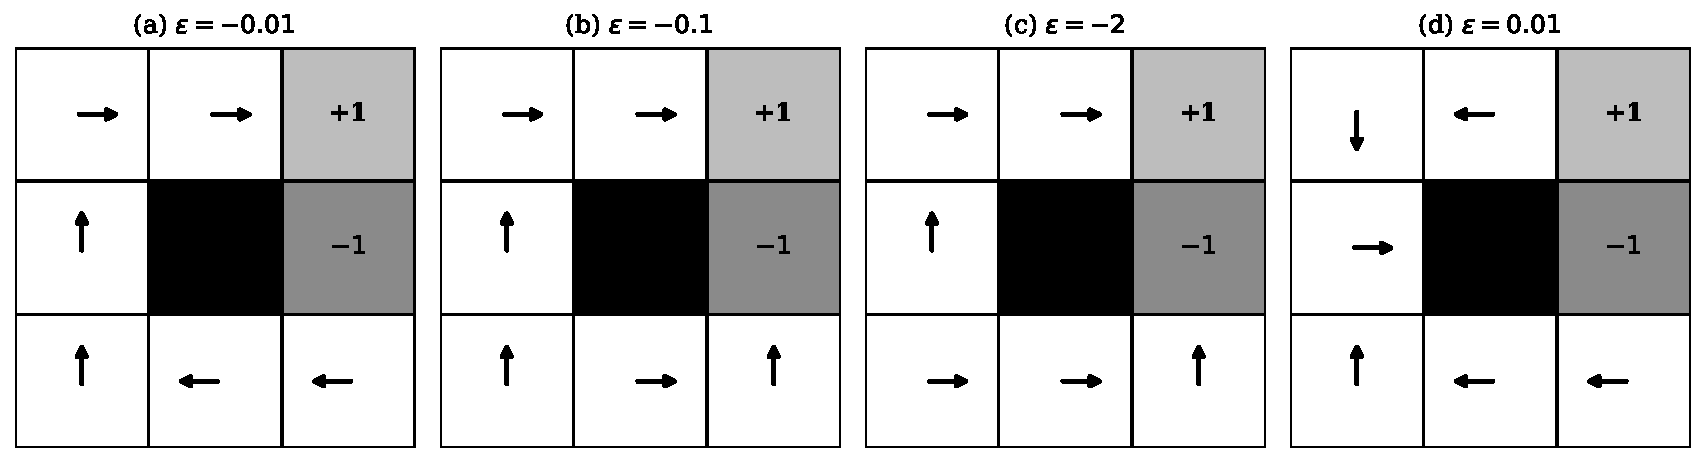
\includegraphics[width=0.95\textwidth]{gridworld_policies}
\end{center}
\textbf{Figure 6.5 (recreated).} Optimal policies for the stochastic
gridworld, for various step penalties $\varepsilon$.
\begin{itemize}
  \item \textbf{(a)} Small negative penalty: the agent acts cautiously,
    taking the long way around to avoid accidentally slipping into the
    $-1$ cell.
  \item \textbf{(b)} Larger negative penalty: the agent is incentivized to
    risk walking past the $-1$ cell to reach $+1$ faster, accepting the
    danger of slipping in.
  \item \textbf{(c)} Extreme negative penalty ($\varepsilon=-2$): life is so
    unbearable that the agent rushes toward \emph{any} terminal cell (even
    $-1$) in as few steps as possible.
  \item \textbf{(d)} A small \emph{positive} reward on every step: the
    agent avoids the terminal cells entirely, hiding behind the wall to
    drag out the episode for as long as possible and maximize the return.
\end{itemize}

\framebreak

\begin{block}{Remark 6.6.6 (Infinitely far-sighted agents may act poorly)}
Optimal policies always exist if $m$ is finite, since then there are only
finitely many policies and $\sup_\pi$ reduces to $\max_\pi$. For $m \to
\infty$, optimal policies continue to exist provided $\Gamma_k < \infty$.
For $\Gamma_k = \infty$ (no discount, infinite horizon), this may no longer
be true: revisiting the delay environment $\nu_{\text{delay}}$ from Figure
6.3 with infinite horizon $m=\infty$ and no discount, the policy $\pi_n$
that takes $n \ge 0$ steps right and then a step upwards achieves value
$V^{\pi_n}_{\nu_{\text{delay}}} = \frac{n+1}{n+2}$, while the policy
$\pi_\infty$ that always steps right achieves
$V^{\pi_\infty}_{\nu_{\text{delay}}} = 0$. So there is no optimal policy:
for any finite $n$ we have $V^{\pi_n}_{\nu_{\text{delay}}} <
V^{\pi_{n+1}}_{\nu_{\text{delay}}}$, and $\pi_\infty$ is the \emph{worst}
policy of all, with
$V^{\pi_\infty}_{\nu_{\text{delay}}} = 0 < \tfrac12 = V^{\pi_0}_{\nu_{\text{delay}}}$.
\end{block}

\framebreak

\textbf{Linearity and convexity.} As a consequence of the linearity of
expectation, the value function is \emph{linear} in the environment: if an
environment $\nu$ can be written as a weighted average of environments
$\nu_i$, then the value function for $\nu$ can also be written as a
(posterior) weighted average of the value functions for the $\nu_i$.
Similarly, the value function is linear in the policy, and the
\emph{optimal} value function is \emph{convex} in the environment.

\begin{block}{Lemma 6.6.7 (Linearity/convexity of $V$ --- informal)}
$V^{\pi,m}_\nu(h_{<t})$ is linear in $\nu$ and $\pi$, and
$V^{*,m}_\nu(h_{<t})$ is convex in $\nu$.
\end{block}

\begin{block}{Example 6.6.8 (Optimal value $V^{*}_\nu$ is not linear in $\nu$)}
Consider a coin flip prediction problem, with $\A=\Ocal=\Rcal=\{0,1\}$, and
two environments $\nu_0, \nu_1$ representing a two-headed and two-tailed
coin respectively. The agent gets reward $1$ for guessing the outcome
correctly, $0$ otherwise:
\[
  \nu_0(e_t|h_{<t}a_t) = \begin{cases}1 & (a_t,o_t,r_t)=(0,0,1)\\1&(1,0,0)\\0&\text{otherwise}\end{cases}
  \qquad
  \nu_1(e_t|h_{<t}a_t) = \begin{cases}1 & (a_t,o_t,r_t)=(0,1,0)\\1&(1,1,1)\\0&\text{otherwise}\end{cases}
\]
\end{block}

\framebreak

Now consider $\nu := \tfrac12\nu_0 + \tfrac12\nu_1$, the environment that
flips a fair coin and rewards $1$ for a correct guess. With no discounting
and horizon $m=1$, \emph{any} strategy in $\nu$ is optimal (no policy can
guess the outcome of a fair coin better than any other), so
$V^{*,m}_\nu(h_{<t}) = \tfrac12$. But since $\nu_0,\nu_1$ are deterministic,
the optimal strategy \emph{knowing which one it is} is to always predict
$i$, so $V^{*,m}_{\nu_1}(h_{<t}) = V^{*,m}_{\nu_2}(h_{<t}) = 1$, which gives
\[
  \tfrac12 V^{*,m}_{\nu_1}(h_{<t}) + \tfrac12 V^{*,m}_{\nu_2}(h_{<t})
  \;=\; 1 \;>\; \tfrac12 \;=\; V^{*,m}_\nu(h_{<t})
\]
hence $V^{*,m}_\nu$ is \emph{not} linear in $\nu$ for $m=1$ (the strict
inequality demonstrates convexity: the average of the optimal values is
strictly larger than the optimal value of the average). This remains true
for $m>1$.
\end{frame}

\begin{frame}[fragile]{Python: Value Iteration on a Small Gridworld}
This computes $V^{*}$ numerically for a $2\times 2$ deterministic
mini-gridworld (a tiny version of Example 6.6.4) via the recursive Bellman
equation, backward from the terminal cells.

\begin{lstlisting}
# Grid layout (row, col), 0-indexed, 2 rows x 2 cols:
#   (0,0) (0,1)=+1
#   (1,0) (1,1)=-1
GOAL, PIT = (0, 1), (1, 1)
REWARDS = {GOAL: 1.0, PIT: -1.0}
CELLS = [(0, 0), (0, 1), (1, 0), (1, 1)]
ACTIONS = {'up': (-1, 0), 'down': (1, 0), 'left': (0, -1), 'right': (0, 1)}

def step(cell, action):
    dr, dc = ACTIONS[action]
    r, c = cell[0] + dr, cell[1] + dc
    if 0 <= r < 2 and 0 <= c < 2:
        return (r, c)
    return cell  # bump into the wall: stay put

gamma = 0.9
V = {c: 0.0 for c in CELLS}
for c in (GOAL, PIT):
    V[c] = REWARDS[c]

for iteration in range(50):
    newV = dict(V)
    for c in CELLS:
        if c in (GOAL, PIT):
            continue
        newV[c] = max(gamma * V[step(c, a)] for a in ACTIONS)
    V = newV

for c in CELLS:
    print(f"V*{c} = {V[c]:.4f}")
\end{lstlisting}

\textbf{What this shows.} Value iteration repeatedly applies the Bellman
optimality equation $V^{*}(c) = \max_a \gamma V^{*}(\text{step}(c,a))$ until
convergence. Running this gives $V^{*}(0,0) = 0.9$ (one step from the goal
via ``right'', so a single discount factor of $\gamma=0.9$) and
$V^{*}(1,0)=0.81$ (two steps from the goal via ``up'' then ``right'',
discounted twice: $\gamma^2=0.81$), matching the intuition that cells
closer to the $+1$ goal have higher optimal value.
\end{frame}

%% ══════════════════════════════════════════════════════════════════════════
\section{6.7 Q-Value}
%% ══════════════════════════════════════════════════════════════════════════

\begin{frame}[allowframebreaks]{6.7 Q-Value}

The value function (Definition 6.6.1) can be extended to an
\emph{action-value} or \emph{Q-value} function, capturing how good it is to
take a specific action $a_t$ given a history $h_{<t}$.

\begin{block}{Definition 6.7.1 (Q-value)}
The Q-value $Q^{\pi,m}_{\nu,\gamma}: \Hcal \times \A \to \mathbb{R}$ of a
policy $\pi$ in an environment $\nu$, given a history $h_{<t}\in\Hcal$,
action $a_t$, horizon $m\ge t$, and discount function $\gamma_t$, is
defined as
\[
  Q^{\pi,m}_{\nu,\gamma}(h_{<t},a_t) :=
  \frac{1}{\Gamma_t}\mathrm{E}^\pi_\nu\!\left[\sum_{k=t}^{m}\gamma_k r_k\,\middle|\,h_{<t}a_t\right]
  = \frac{1}{\Gamma_t}\sum_{e_t}\nu(e_t|h_{<t}a_t)\sum_{h_{t+1:m}}\nu^\pi(h_{t+1:m}|h_{1:t})\sum_{k=t}^m\gamma_k r_k
\]
If $t>m$ or $\Gamma_t=0$ we define $Q^{\pi,m}_{\nu,\gamma}(h_{<t},a_t):=0$.
The optimal Q-value function is defined as
\[
  Q^{*,m}_\nu(h_t a_t) := \sup_\pi Q^{\pi,m}_\nu(h_ta_t) = Q^{\pi^{*,m},m}_{\nu,\gamma}(h_ta_t)
\]
\end{block}

\textbf{Plain-English explanation.} $Q^{\pi,m}_{\nu,\gamma}(h_{<t},a_t)$
answers ``how good is it to take action $a_t$ right now (given history
$h_{<t}$), and then follow policy $\pi$ afterward?''. It differs from the
value function $V$ only in that the very next action is \emph{fixed} to
$a_t$, rather than chosen by $\pi$; everything afterward still follows
$\pi$.

\framebreak

\begin{block}{Theorem 6.7.2 (Bellman equations)}
If policy $\pi$ and environment $\nu$ are (proper) probability measures,
then
\begin{align}
  Q^{\pi,m}_{\nu,\gamma}(h_{<t},a_t) &= \frac{1}{\Gamma_t}\sum_{e_t}\nu(e_t|h_{<t}a_t)
  \big[\gamma_t r_t + \Gamma_{t+1}V^{\pi,m}_{\nu,\gamma}(h_{1:t})\big] \tag{6.7.3}\\
  V^{\pi,m}_{\nu,\gamma}(h_{<t}) &= \sum_{a_t}\pi(a_t|h_{<t})\,Q^{\pi,m}_{\nu,\gamma}(h_{<t},a_t) \tag{6.7.4}
\end{align}
Both equations hold for all policies, including optimal policies
$\pi^{*,m}_\nu$, for which (6.7.4) reduces to
\[
  V^{*,m}_{\nu,\gamma}(h_{<t}) = \max_{a_t} Q^{*,m}_{\nu,\gamma}(h_{<t},a_t) \tag{6.7.5}
\]
\end{block}

\textbf{Plain-English explanation.} Equation (6.7.3) says: the Q-value of
taking action $a_t$ equals the immediate discounted reward $\gamma_t r_t$
plus the (rescaled) value of wherever you land next, averaged over the
environment's randomness in producing $e_t$. Equation (6.7.4) says: the
value of a history equals the average Q-value over the actions the policy
might take, weighted by how likely the policy is to take each one. For the
\emph{optimal} policy, (6.7.5) simplifies this to just taking the best
action's Q-value, since an optimal policy always picks the action that
maximizes $Q^{*}$.

\framebreak

\textbf{Proof sketch.} \emph{(i)} Plugging the explicit representation
\[
  V^{\pi,m}_{\nu,\gamma}(h_{1:t}) = \frac{1}{\Gamma_{t+1}}\sum_{h_{t+1:m}}\nu^\pi(h_{t+1:m}|h_{1:t})\sum_{k=t+1}^m\gamma_k r_k
\]
from Definition 6.6.1 into the right-hand side of (6.7.3) and rearranging
terms, exploiting $\sum_{h_{t+1:m}}\nu^\pi(h_{t+1:m}|h_{1:t})=1$, recovers
Definition 6.7.1. \emph{(ii)} Inserting the sum representation of $Q$ from
Definition 6.7.1 into (6.7.4) and using the definition of $\nu^\pi$ leads to
the sum representation of $V$ from Definition 6.6.1. \emph{(iii)} Let
$A_t := \operatorname{argmax}_{a_t}Q^{*,m}_{\nu,\gamma}(h_{<t},a_t)$ be the
set of $Q^{*}$-maximizing actions. Clearly
$\sum_{a_t}\pi(a_t|h_{<t})Q^{*,m}_{\nu,\gamma}(h_{<t},a_t)$ is maximized
with respect to $\pi$ if and only if $\pi(a_t|h_{<t})=0$ for $a_t \notin
A_t$, i.e.\ iff $\pi(a_t|h_{<t}) = \pi^{*,m}_\nu(a_t|h_{<t})$ for some
$\pi^{*,m}_\nu \in \Pi^{*,m}_\nu(h_{<t})$. For such $\pi$, the expression
reduces to $\max_{a_t}Q^{*,m}_{\nu,\gamma}(h_{<t},a_t)$.

\vspace{0.15cm}
\textbf{Consequence: a deterministic optimal policy always exists.} For
deterministic policies $\pi$, (6.7.4) reduces to
$V^{\pi,m}_{\nu,\gamma}(h_{<t}) = Q^{\pi,m}_{\nu,\gamma}(h_{<t},\pi(h_{<t}))$.
By (6.7.5), among the set of optimal policies there is always a
deterministic one: choose any deterministic $\pi$ with $\pi(h_{<t})=a_t$
for any $a_t$ that maximizes $Q^{*,m}_{\nu,\gamma}(h_{<t},a_t)$.

\framebreak

\begin{block}{Lemma 6.7.6 (Contraction property of (Q-)values)}
For $t \le m$,
\[
  \sup_{h_{<t}}\big|V^{\pi,\infty}_\nu(h_{<t}) - V^{\pi,m}_\nu(h_{<t})\big|
  \;\le\; \sup_{h_{<t}a_t}\big|Q^{\pi,\infty}_\nu(h_{<t},a_t) - Q^{\pi,m}_\nu(h_{<t},a_t)\big|
\]
\[
  \le\; \frac{\Gamma_{t+1}}{\Gamma_t}\sup_{h_{1:t}}\big|V^{\pi,\infty}_\nu(h_{1:t})-V^{\pi,m}_\nu(h_{1:t})\big|
  \;\le\; \cdots \;\le\; \frac{\Gamma_{m+1}}{\Gamma_t}
\]
If $\nu$ is a semimeasure this remains true iff $V,Q$ are \emph{defined}
via the recursion in Theorem 6.7.2. The bounds also remain true if all
$\pi$ are replaced by $*$, i.e.\ the optimal policies $\pi^{*}_\nu$ and
$\pi^{*,m}_\nu$.
\end{block}

\textbf{Plain-English explanation.} This says the gap between using the
full infinite-horizon value/Q-value and a finite-horizon truncation at $m$
shrinks the further out the horizon reaches, bounded by the ratio
$\Gamma_{m+1}/\Gamma_t$ (which goes to zero as $m\to\infty$, for
time-consistent, summable discounts). In other words, truncating far
enough into the future barely changes anything.

\vspace{0.15cm}
\textbf{Caution: fails for improper semimeasures unless recursively
defined.} A counter-example: let $\nu$ be a proper measure on $h_{<m}$
always giving reward $1$, and $\nu(h_{<t})\equiv 0$ for $t>m$. Then for all
$t \le m$ we have $V^{\pi,m}_\nu(h_{<t})=1$ but $V^{\pi,\infty}_\nu(h_{<t})=0$.

\framebreak

\textbf{Computing optimal values and policies.} Given an exact model of the
environment $\mu$, and history $h_{<t}$ so far, the optimal action to take
is an action $a_t$ which maximizes $Q^{*,m}_\mu(h_{<t},a_t)$. Therefore, to
find this optimal action, the expectation in Definition 6.7.1 must be
evaluated. Assuming $\mu$ can be computed in time $O(1)$, computing this
expectation naively via the sum representation in Definition 6.7.1 takes
$O((m-t)\cdot(|\Ocal|\cdot|\A|\cdot|\Rcal|)^{m-t})$ time. This makes the
computation intractable for all but the smallest observation $\Ocal$,
action $\A$, and reward spaces $\Rcal$ and horizons $m$.

\vspace{0.15cm}
Finding the optimal action by maximizing $Q^{*,m}_\mu(h_{<t}a_t)$ with
respect to $a_t$ in this form is circular, since $Q^{*,m}$ relies on an
optimal policy $\pi^{*}$ in its definition, and if we already have an
optimal policy, we can just query it directly. The theoretical remedy is to
compute the last expression in Lemma 6.6.3, giving the optimal action:
\[
  a_t := \operatorname*{argmax}_{a_t\in\A}\sum_{e_t\in\Ecal}\max_{a_{t+1}\in\A}\sum_{e_{t+1}\in\Ecal}
  \cdots\max_{a_m\in\A}\sum_{e_m\in\Ecal}\prod_{k=t}^m\nu(e_k|h_{<k}a_k)\sum_{k=t}^m\gamma_kr_k
  \tag{6.7.7}
\]
This nested max/sum expression is called the \emph{expectimax tree} or
\emph{expectimax algorithm}.

\framebreak

\textbf{Plain-English explanation.} Expectimax alternates $\max$ (the
agent's turn: pick the best action) with $\sum$ (the environment's turn:
average over all possible random percepts), all the way out to horizon
$m$. It is a brute-force way to find the truly optimal action, but its cost
grows exponentially with the remaining horizon $m-t$, which is why it is
only practical for very small problems.

\vspace{0.2cm}
\textbf{Bridge to practical RL.} The recursive Bellman expressions from
Theorem 6.7.2 often form the basis for more efficient and practical MDP RL
algorithms, which learn the optimal Q-value function directly via
techniques such as Q-learning, without ever exhaustively expanding the
expectimax tree. From an approximation of the $Q^{*}$ values, an
approximately optimal policy can be recreated by
$\pi^{*,m}(h_{<t}) = \operatorname{argmax}_{a_t}Q^{*,m}(h_{<t},a_t)$.
\end{frame}

\begin{frame}[fragile]{Python: Expectimax and the V/Q Bellman Recursion}
This example computes $Q^{*}$ and $V^{*}$ via the expectimax recursion
(6.7.7)/(6.7.5) for a tiny 2-step stochastic environment, then checks that
the Bellman equations (6.7.3)--(6.7.5) hold numerically.

\begin{lstlisting}
# Two actions 'L','R'. Percept space just carries a reward in {0,1}.
# nu(e|h,a): probability of reward 1 given action a (independent of history).
reward_prob = {'L': 0.4, 'R': 0.6}
ACTIONS = ['L', 'R']
gamma = 0.9  # geometric discount, gamma_k = gamma^k

def Q_star(t, m):
    """Optimal Q-value at remaining horizon (m-t) steps, Q*(a) for each a."""
    if t > m:
        return {a: 0.0 for a in ACTIONS}
    q = {}
    for a in ACTIONS:
        p = reward_prob[a]
        # E[reward now] + gamma * E[V*_{t+1}]  (Eq. 6.7.3, unnormalized)
        v_next = V_star(t + 1, m)
        q[a] = p * (1.0 + gamma * v_next) + (1 - p) * (0.0 + gamma * v_next)
    return q

def V_star(t, m):
    if t > m:
        return 0.0
    return max(Q_star(t, m).values())   # Eq. 6.7.5

m = 2
for t in [0, 1, 2]:
    q = Q_star(t, m)
    v = V_star(t, m)
    print(f"t={t}: Q*(L)={q['L']:.4f}  Q*(R)={q['R']:.4f}  V*={v:.4f}  "
          f"best action={max(q, key=q.get)}")
\end{lstlisting}

\textbf{What this shows.} At every time step, $Q^{*}(\text{'R'}) >
Q^{*}(\text{'L'})$ since action \texttt{'R'} has a higher reward
probability (0.6 vs.\ 0.4), so the optimal deterministic policy always
chooses \texttt{'R'} --- consistent with the theorem that a deterministic
optimal policy always exists (Theorem 6.7.2). The code also numerically
verifies $V^{*}(h_{<t}) = \max_{a_t}Q^{*}(h_{<t},a_t)$ (Eq.\ 6.7.5) by
construction, since \texttt{V\_star} is literally defined as the max over
\texttt{Q\_star}.
\end{frame}

%% ══════════════════════════════════════════════════════════════════════════
\section{6.8 Exercises}
%% ══════════════════════════════════════════════════════════════════════════

\begin{frame}[allowframebreaks]{6.8 Exercises}

The book lists the following exercises for Chapter 6 (difficulty ratings in
brackets, e.g.\ [C15] means ``Coding/Computation difficulty 15'' on the
book's own scale):

\begin{enumerate}
  \item [C03] Give an example of an environment where all policies are
    optimal.
  \item [C15] In Section 6.3, POMDPs are claimed to be a specific instance
    of history-based RL. Prove this claim. In particular, given that the
    policy and environment both have access to the entire interaction
    history, how can we construct the environment so that it has access to
    the true underlying state, but the policy does not?
  \item [C20] Show that the conditional
    $\nu^\pi(e_{1:m}|a_{1:m}) := \nu^\pi(h_{1:m})/\sum_{a_{1:m}}\nu^\pi(h_{1:m})$
    (Definition 6.1.5) is different from the chronological
    $\nu(e_{1:m}||a_{1:m})$ (Definition 6.3.1), and elaborate in which ways,
    and why this is important. For instance, show that
    $\sum_{e_m}\nu(e_{1:m}||a_{1:m}) = \nu(e_{<m}||a_{<m})$ is independent
    of $a_m$, while $\sum_{e_m}\nu^\pi(e_{1:m}|a_{1:m}) \ne
    \nu^\pi(e_{<m}|a_{<m})$ depends on $a_m$.
  \item [C10] Give some examples of undesirable behavior that can result
    from using: no discount, negative discount, monotonically increasing
    discount.
  \item [C20] Derive the expressions for $H_t(\epsilon)$ and $\Gamma_t$ in
    Table 6.4.
  \item [C10] Show that in Example 6.5.3 with geometric discounting
    $\gamma$, the agent will choose to walk $k^{*}-1$ steps right, and then
    on time step $k^{*}$ walk up, where
    $k^{*}=\operatorname{argmax}_{k\ge1}\{\gamma^{k-1}\tfrac{k}{k+1}\}<\infty$.
  \item [C15] Prove the equivalence of the expectation and sum
    representations of the (Q-)value functions in Definitions 6.6.1 and
    6.7.1.

\framebreak
  \item [C15i] Derive the explicit representations of the value function in
    Lemma 6.6.3.
  \item [C15] Derive explicit representations of the Q-value function
    analogous to Lemma 6.6.3.
  \item [C20] Complete the proof details for Theorem 6.7.2.
  \item [C18] Show that the Bellman (optimality) equations of Theorem 6.7.2
    also hold for $m \to \infty$.
  \item [C20] Formulate the claims in Lemma 6.6.7 precisely and prove them.
    (Hint: this exercise becomes easier after reading Section 7.2, using
    the posterior $w(\nu|h_{<t})$.)
  \item [C20i] Prove that for finite action sets $\A$ and bounded reward
    space $\Rcal$ and $\Gamma_t < \infty$, an optimal policy and optimal
    actions for $m\to\infty$ indeed exist. Show that these conditions are
    necessary.
  \item [C25i] Show that $\varepsilon_t$-optimal policies and actions always
    exist, even for countable action spaces $\A$, for any choice of
    $\varepsilon_t$, e.g.\ constant $\varepsilon_t=\varepsilon$ or
    decreasing $\varepsilon_t=o(1)$.
  \item [C15] Prove that if $\pi \in \Pi^{*}(\epsilon)$ then $\pi \in
    \Pi^{*}(h_{<t})$ (on histories which $\pi$ can generate).
  \item [C22] In place of a discount function, one can assume that the sum
    of rewards output by the environment $\nu$ is finite. Show this is a
    strict generalization of having a discount function (e.g.\ all discount
    functions are contained in this setup, as well as setups which cannot
    be described using discount functions).
\end{enumerate}
\end{frame}

%% ══════════════════════════════════════════════════════════════════════════
\section{6.9 History and References}
%% ══════════════════════════════════════════════════════════════════════════

\begin{frame}[allowframebreaks]{6.9 History and References}

This chapter is based on material from [Hut05b] and [Lei16b, Chp.4].

\begin{block}{Books on reinforcement learning}
The reinforcement learning book by Sutton and Barto [SB18] requires no
background knowledge, and describes from scratch the field of
reinforcement learning. It covers bandit problems and various methods of
attack for MDPs: exact solutions, tabular learning, and approximate
methods, though more state-of-the-art approaches using deep learning are
not covered. Tougher and more rigorous books by Bertsekas (and Tsitsiklis)
[BT96, Ber19, Ber20] provide all the convergence proofs that Sutton and
Barto gloss over. In-depth surveys of reinforcement learning can be found
in [KLM96, Sze10, GMPT15, MBJ20]. Additional useful resources for studying
reinforcement learning include the books [KV86, WvO12, AJKS22, Mey22,
Pla22]. See the book's Section 14.6 for more RL ideas and algorithms mostly
not (yet) covered in (m)any of these books.
\end{block}

\begin{block}{Bandit problems}
Bandit problems (MDPs with only a single state) are still complex enough to
demonstrate trade-offs between exploitation and exploration [BF85, BK97,
ACBF02], and are covered in great depth in [LS20].
\end{block}

\framebreak

\begin{block}{Rewards}
The reward hypothesis (Assumption 6.2.1) is the core assumption on which
reinforcement learning relies. This hypothesis cannot be proven either way
(goals and purposes are not formally defined terms), though there is much
work both in support of it [SSPS21], and some in opposition to it
[VSK$^{+}$22]. Many problems often have multiple goals to simultaneously
fulfil, and these goals can be in conflict --- for example, a self-driving
car needs to balance minimizing time to the destination against passenger
safety, road rules, cost of fuel, etc. It is not immediately clear how to
aggregate these competing goals into a single scalar reward, especially if
the relative trade-off between the goals is not fixed (some passengers
might be in a rush; others might want to take things slow). Such problems
are studied in \emph{multi-objective reinforcement learning} (MORL)
[HR$^{+}$22]; a survey can be found in [RVWD13].
\end{block}

\vspace{0.1cm}
Learning is often more difficult in environments with sparse rewards.
Imitation learning [CHN22] or shaping the reward can help, but usually
requires extra domain knowledge [Mat94]. Ideally, the reward should be
shaped so as to leave the optimal policy unchanged, but easier for the
agent to find [NHR99]. For environments where the agent is trying to reach
a goal state, one work [TZXS19] describes a shaped reward based on a
measure of distance from the goal, while avoiding getting trapped in local
optima. A proxy goal can also be chosen, often a goal that encourages the
agent to seek new and novel experiences: Orseau's Knowledge-Seeking Agent
(KSA) [OLH13] is covered later in the book (Section 9.3), which tries to
gather information about the environment it is in; Burda [BESK18] notes
that KSAs can perform well on complex environments, but can also focus
their attention on sources of noise.

\framebreak

\begin{block}{Multi-agent RL}
Some environments contain an opponent to play against (such as chess).
Often, \emph{self-play} is used, where the agent also plays the role of its
own opponent. This was used to great success to train agents to play
\emph{backgammon} [Tes94, T$^{+}$95] and \emph{Go} [SH$^{+}$16]. A survey of
self-play RL can be found in [DZ21]. To encode two agents playing against
each other in the book's agent-environment framework, each agent considers
the other to be part of the environment with which it interacts (covered
later in Chapters 10 and 11). \emph{Multi-Agent Reinforcement Learning}
(MARL) covers many agents interacting together in an environment, often
with adversarial rewards to incentivize competition, or aligned rewards to
incentivize cooperation. A survey of MARL is provided in [HLKT19].
\end{block}

\begin{block}{Illegal actions}
Commonly used methods to deal with illegal moves in games include issuing a
larger penalty than the penalty for losing a game [WPH22], or having the
illegal action have no effect [H$^{+}$02]. For stochastic policies, one can
resample until a legal move is obtained (for black-box policies), or zero
the probabilities for illegal moves and renormalize [SH$^{+}$16]. The
former two methods do not require leaking information about the
environment to the agent, whereas the latter method of tampering with the
distribution over actions requires domain knowledge of the environment.
\end{block}

\framebreak

\begin{block}{Time-discounting}
Time discounting is a trick used to ensure the reward sum is finite, and
often justified based on an argument appealing to the finite lifetime of an
agent [Soz98], or that in practice most humans choose immediate
gratification over a marginally larger reward later. On the other hand,
humans often forgo immediate gratification for sufficiently larger rewards
later. The famous ``marshmallow test'' [ME70] provided one of the earliest
studies into how children discount rewards, offering them one marshmallow
now, with the offer to provide two if the child could resist eating the
first for a period of time.
\end{block}

\vspace{0.1cm}
[LH11c] introduced the generalized discount (Definition 6.4.1) which can
depend on the age of the agent. A complete characterization of when it is
time-(in)consistent can be found in [LH14b]; they also show the existence
of a rational policy for an agent that knows its discount function is
time-inconsistent.

\vspace{0.1cm}
However, most of the time in RL, the agent is immortal, and does not have
the option to ``invest'' its reward. Schwartz explores an undiscounted
method of measuring the performance of a policy similarly to a Ces\`aro sum
[Sch93]. [LH07c, Sec.3] avoids pre-commitment to any particular discounting
by letting the environment decide how to discount. Pitis justifies a set of
axioms that a discount should satisfy, and derives a form of discounting
that can be state-dependent, generalizing the typical fixed discount
methods [Pit19]. Low discount factors can speed up convergence [BT96], but
lead to poor performance. Van Seijen [VSFT19] hypothesizes that this is due
to the size of the \emph{action-gap} (the difference in value between the
best and second-best actions), and proposes a method to make the
action-gaps more homogeneous by applying updates in logarithmic space.
Reinforcement learning can serve as an idealized setting to study how
discounting can lead to (sub)optimal/(un)healthy behavior [SVS$^{+}$14].

\vspace{0.1cm}
One can show that (past) undiscounted truncated values are asymptotically
equivalent to (future) untruncated discounted values, provided the
effective horizon increases unboundedly [Hut06a]. Truncated Value Learning
(TVL) mimics discounting by learning multiple undiscounted truncated value
functions [ASDH24]; it simultaneously learns values for \emph{all}
(summable) discount functions.
\end{frame}

\end{document}
